\title{ Unions of Balls and Configuration Space }
\author{
        Yinan Zhang\\
        Department of Computer Science\\
        Dartmouth College\\
        Hanover, New Hampshire 03755, US
        \and
        Devin Balkcom \\
        Department of Computer Science\\
        Dartmouth College\\
        Hanover, New Hampshire 03755, US
}
\date{\today}

\documentclass[11pt]{article}
\usepackage{amsmath}
\usepackage{amsfonts}
\usepackage{graphicx}
\DeclareGraphicsExtensions{.pdf,.png,.jpg, .gif}
\usepackage{algpseudocode}

\newtheorem{theorem}{Theorem}[section]
\newtheorem{lemma}[theorem]{Lemma}
\newtheorem{definition}[theorem]{Definition}


\begin{document}
\maketitle

\begin{abstract}
Covering both the configuration space and represent the right topology is hard to achieve at the same time with traditional sampling-based motion planning algorithms, such as Probabilistic Roadmap and Rapidly-Exploring Random Tree. In this paper, we proposed a method that is able to cover near optimal path and study the shape and topology of configuration space. 
\end{abstract}

\section{Introduction}
This is time for all good men to come to the aid of their party!

%%%%%%%%%%%%%%%%%%%%%%%%%%%%%%%%%%%%%%%%%%%%%%%%%%%%%%%%%%%%%%%%
%	Introducing Related Work
%
%%%%%%%%%%%%%%%%%%%%%%%%%%%%%%%%%%%%%%%%%%%%%%%%%%%%%%%%%%%%%%%%

\section{Related Work}\label{related work}

\indent\indent In this section, we first discuss the basics of sampling-based motion planning and the method of sampling on medial axis. With the information of positions and their clearance in c-space, we have samples as spheres. We then discuss the dual shapes of the union of balls which plays an important role in understanding the shape of c-space and its topology. Some works on graph theory and topology will finally be introduced.

%====================================
% Sampling Based Motion Planning
%====================================

\paragraph{A} \emph{Sampling-based Motion Planning} \hfill \\
\indent A robot is a movable object whose state can be described by $n$ parameters, or \emph{degrees of freedom} ($DOFs$). A point $<x_1, x_2, ..., x_n>$ in a n-dimensional space uniquely defines the configuration of a robot. Such space is called \emph{"Configuration Space"} or \emph{"C-space"}  ($C$). The subset of all feasible configurations is called the \emph{free space} (\emph{$C_{free}$}), while $C_{obst} = C \setminus C_{free}$ is the union of all infeasible configurations. \cite{UMAPRM} Path planning will generally be viewed as a search in a metric space $X$ for a continuous path from an initial state $x_{init}$ to a goal region $X_{goal} \subset X$. For a standard problem, $X = C$. \cite{RRT} What needs to be pointed out is that \emph{C-space} is very different from workspace which is usually formed by polygons. The shape of \emph{C-space} is usually unknown to us, unless the robot is a point. 

\indent Sampling-based algorithms have been very successful and have seen many applications in industry for planning in high dimension space. Probablistic Roadmap \cite{PRM} and Rapidly-Exploring Random Tree \cite{RRT} are two outstanding methods. The basic idea under these methods is to randomly sample feasible configurations in \emph{C-space} and connect nearby valid samples as edges to construct a graph or tree structure, which careless about the dimension problem. By connecting start and goal configurations to the roadmap, a graph search, e.g., A*, can be performed to extract a near optimal solution path.

\indent One disadvantage of these methods is that we can't study the topological structure of C-space using only the data structures constructed.

%====================================
% Sampling on medial axis
%====================================
\paragraph{B} \emph{Medial Axis Sampling} \hfill \\
\indent A simpler method that maintains the topology of \emph{C-space} but doesn't cover near optimal path is medial axis sampling. Medial Axis is also called Generallized Voronoi Diagram. The medial axis $MA(F)$ of free space $F$ is a strong deformation retract of $F$, which means $F$ can be continuously deformed onto $MA(F)$ while maintaining its topological structure. However, medial axis is hard to compute explicitly.

\indent In Figure \cite{Book}, sec. 5.6.3, Steven LaValle defined Medial Axis as "Let $(X, \rho)$ be a metric space. Let a \emph(maximal ball) be a ball $B(x,r) \subseteq X$ such that no other ball can be a proper subset the centers of all maximal balls trace out a one-dimensional set of points referred to as the \emph{medial axis}".  

\indent Mapping a pair of points $A$ and $B$ in free space onto $MA(F)$, there is a path between $A$ and $B$ if and only if there is a path between their images on $MA(F)$. Such path has a very nice property of the largest clearance from obstacles.

\indent Steven A. Wilmart \cite{MAPRM} sampled on the medial axis of free space to build up a probabilistic roadmap planner. He also showed that "it is possible to efficiently retract a configuration, free or otherwise, onto the medial axis of the free space without having to compute the medial axis explicitly".

\indent The basic idea of the algorithm proposed in \cite{MAPRM} is: given a point $A$ and its nearest point on the boundary of obstacles $A'$, a ray start from $A$ with direction $\overrightarrow{A'A}$ will always intersect with $MA(F)$.

\indent This method results in sampling more nodes in narrow corridors, which is beneficial for improving performance on problems requiring traversal of such corridors.

\indent However, such property makes the sampling method biased heavily towards certain portions of the medial axis. These biased property tend to ignore more critical parts of the space: large open free space. Sampling uniformly on the medial axis is sometimes more helpful.

\indent Hsin-Yi (Cindy) Yeh \cite{UMAPRM} solved this problem by putting some random "sticks" with random directions in free space. Any surfaces will intersect uniformly with these sticks, thus searching on sticks to find points that intersect with medial axis will give nodes uniformly distributed on the medial axis.

\indent Figure \ref{fig:Medial Axis} visualizes the shape of medial axis of a rectangle.

\begin{figure}
	\center{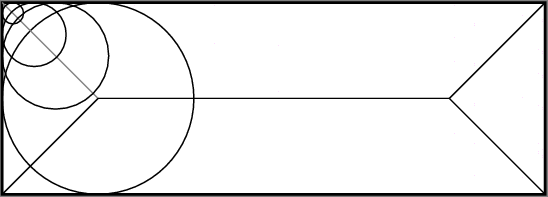
\includegraphics[scale=0.35]{./pics/MA.png}}
	\caption{\label{fig:Medial Axis} Sampling on the Medial Axis of a rectangle space.\cite{Book}}
\end{figure}

%====================================
% Dual shapes of unions of balls
%====================================

\paragraph{C} \emph{Dual Shapes of Unions of Balls} \hfill\\
\indent Approximating the shape of an unknown area to study its properties is a very commonly used method. We have seen many such ideas in the study of biogeometry. As for robotics, a few people began to notice the achievements from biogeometry study and tried to apply similar methods to study the shape of \emph{C-space}. 

\indent Zoe McCarthy \cite{PathNonexistance} used samples generated by PRM to form the $\alpha$-shape of \emph{C-space}. She then proved there doesn't exist a path between a pair of configurations by proving they are in two different disconnected components of the shape. She declared it was the first time $\alpha$-shape is being used in motion planning.

\indent Define a \emph{simplicial complex} $D$: a collection of simplices such that if $\bigtriangleup_T \subseteq D$ ( $\bigtriangleup_T$ is the convex hull of $T$ ), then if $U \subseteq T$, we have $\bigtriangleup_U \subseteq D$ and also that the intersection of two simplices in $D$ is either empty or another simplex in $D$. The $\alpha$-shape of a set of points $S$ is a generalization of the convex hull of those points. \cite{PathNonexistance}. H. Edelsbrunner first introduced them in \cite{PointSetShape}. By choosing different value of the one parameter $\alpha$, we can have a family of shapes with the same set of points. An example of $\alpha$-shape is in Figure \ref{fig:Alpha-shape}.

\indent Choosing the best $\alpha$ value could be a bothering work. Assuming weighted points in the point set, by using a generalization of the Delaunay Triangulation, the Regular Triangulation, we can construct another shape using weights as flexible $\alpha$'s. Points with weights can be considered as balls. H. Edelsbrunner gave us this idea in \cite{DualShape}. Such shapes are also called Dual Shapes or Dual complex of unions of balls. The weighted $\alpha$-shape captures the topology of the union of balls with different radii. Figure \ref{fig:Dual Shape} shows an example of such weighted $\alpha$-shape.

\begin{figure}
	\center{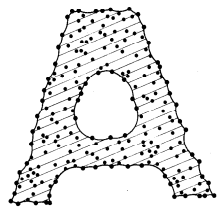
\includegraphics[scale=0.7]{./pics/alphaShape.png}}
	\caption{\label{fig:Alpha-shape} An example of $\alpha$-shape. \cite{PointSetShape}}
\end{figure}

\begin{figure}
	\center{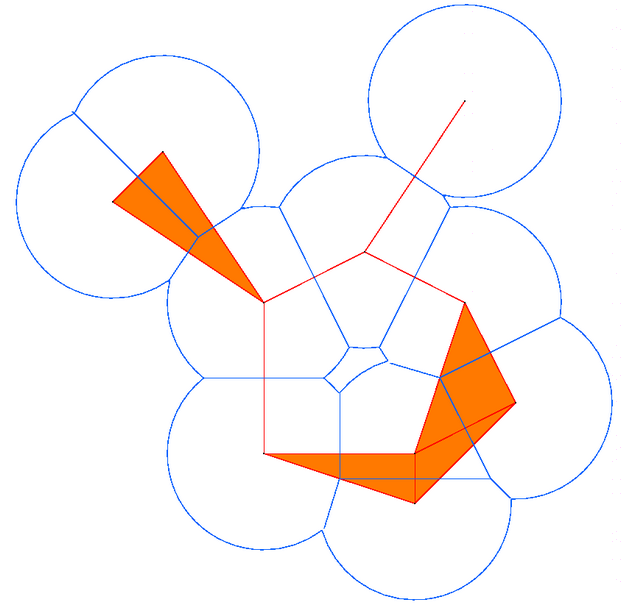
\includegraphics[scale=0.30]{./pics/dualshape.png}}
	\caption{\label{fig:Dual Shape} An example of weighted $\alpha$-shape for a union of balls. \cite{DualShape}}
\end{figure}

%====================================
% Betti Numbers
%====================================
\paragraph{D} \emph{Betti Numbers} \hfill \\
\indent In algebraic topology, the Betti Numbers are used to distinguish topological spaces based on the connectivity of n-dimensional simplicial complexes. Informally, the \emph{n-th} Betti number ($\beta_n$) represents the rank of the \emph{n-th} homology group, which tells us the maximum number of cuts that can be mad before diving a surface into two pieces. \cite{betti wiki}

\indent An example of Betti numbers will be a torus. Figure \ref{fig:Torus}

\indent The first betti number of a graph is very easy to compute. Given a graph $G$, with $n$ vertices, $m$ edges and $k$ components. It's 1st betti number is:

$\beta_1 = m - n + k$

\indent This can be proved straightforwardly by mathematical induction on the number of edges. A new edge either increments the number of 1-cycles or decrements the number of connected components. \cite{betti wiki}

\indent H. Edelsbrunner introduced a way to compute $n-th$ Betti number in \cite{Edel Book}, where he uses gaussian ellimination to compute the betti numbers with adjacency matrix.

\indent Vanessa Robins \cite{alpha betti} provided more detailed explains and proofs on computing betti numbers. What's more, she put more thoughts on computing betti numbers for alpha shapes.

\begin{figure}
	\center{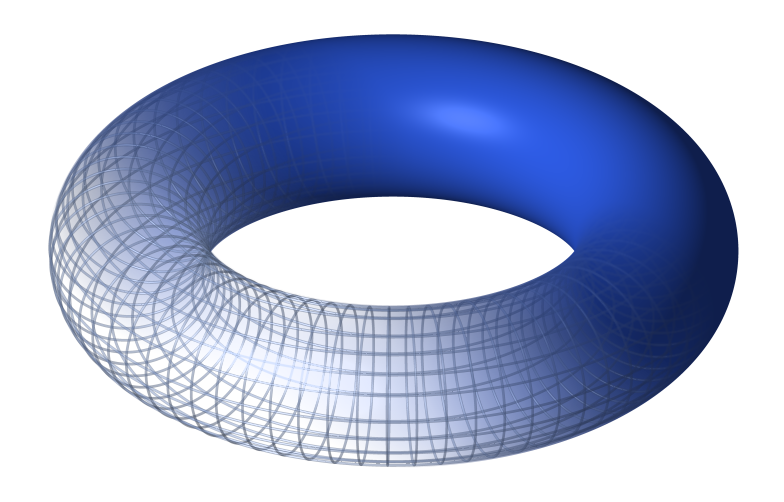
\includegraphics[scale=0.26]{./pics/Torus.png}}
	\caption{\label{fig:Torus} The torus has one connected component($\beta_0$), two circular holes ($\beta_1$,the one in the center and the one in the middle of the "donut"), and one two-dimensional void ($\beta_2$, the inside of the "donut").\cite{betti wiki}}
\end{figure}


%%%%%%%%%%%%%%%%%%%%%%%%%%%%%%%%%%%%%%%%%%%%%%%%%%%%%%%%%%%%%%%%
%	Introduction to Our Algorithm
%
%%%%%%%%%%%%%%%%%%%%%%%%%%%%%%%%%%%%%%%%%%%%%%%%%%%%%%%%%%%%%%%%

\section{Our Method}\label{method}

\indent \indent Traditionally, sampling based algorithms will build a graph for configuration space. These kind of graphs are proved to be able to find near optimal path, but can hardly be used to analysis the topology of paths. We want to to build a stronger representation of c-space that is both able to cover optimal path and study the topological structure of c-space. In this section, we are trying to solve the problem in 2D and answer the question "Is two paths in the same homotopy class" as a start point of using our method to study the topology of \emph{C-space}. We will first give the outline of the algorithm, and explain each step in detail. 

%====================================
% Algorithm outline
%====================================
\paragraph{A} \emph{The Algorithm outline} \hfill \\
\indent Before starting introducing our algorithm, we firstly clarify some preliminary tools we can have: We are sampling in $(X, \rho)$ metric space. Let $x$ be a configuration in $X$(usually \emph{C-space}), $\rho(x)$ gives the clearance of configuration $x$. By \emph{"clearance"}, we mean its (estimated) distance to the nearest obstacles. Ball $B(x, \rho(x))$ is referred as a $"sample"$ in the rest of the section. We make no assumption of the shape of obstacles regions in \emph{C-space}. 

\indent The algorithm is shown in Figure \ref{fig:Algo}. It has four phases. The first phase is to generate some random configurations in \emph{C-space}, like all other sampling-based planning algorithms do, and keep only those feasible ones. Every feasible configuration will be kept until the third phase. ($randomConfig$ keep unchanged.) In the second phase, we will sample balls centered on medial axis first and then try to cover the left area of $C_{free}$. Samples on the medial axis $MA(C_{free})$ will be used in phase three to construct the dual shape that captures the topology of $C_{free}$. After simplifying the dual shape, we will have a roadmap while maintaining the topological structure. Phase four break the topology roadmap into pieces such that no two piece can be merged without forming a loop. 

\indent We will now explain each phase in detail.

%%%%%%%%%%%%%%%%================================================>>>>>>>>>>>>>>>>>>>>>>>>>>>>>>
%%%%%%  We need to name our algorithm
%%%%%%  Seriously
%---------------------------------------------------------------------------------------------
\begin{figure}
  \begin{algorithmic}[1]
  \Function{WeNeedAGoodName}{\emph{C-space}}
  
    // Phase One
    \indent \State $randomConfigs \gets SampleRandomConfigurations( \emph{C-space}, number )$ 

    // Phase Two
    \indent \State $maSamples \gets SampleOnMedialAxis( randomConfigs )$
    \indent \State $regSamples \gets SampleLeftArea(maSamples, randomConfigs)$

    // Phase Three
    \indent \State $dualShape \gets WeightedAlphaShape( some smaples )$
    \indent \State $topologyRoadmap \gets Retract(dualShape)$ 

    // Phase Four
    \indent \State $brokenRoads \gets BreakGraph( topologyRoadmap )$
    
    \indent 
	
  \EndFunction
  \end{algorithmic}
  \caption{\label{fig:Algo} Algorithm Outline}
\end{figure}

%====================================
% Covering c-space
%====================================
\paragraph{B} \emph{Sampling in C-space} \hfill \\
\indent As pointed out in Figure \ref{fig:Algo}, this phase has two parts: Sampling on medial axis, and sampling the rest of free space. 

\indent Sampling on medial axis is well studied in \cite{MAPRM} and \cite{UMAPRM}. Besides the positions of configurations, we also keep the clearance of each configuration, thus have some balls, or samples. We also require that no new ball, when sampling, is allowed to be centered inside any existing one. For details of the algorithms, please refer to these two papers. One thing worth our notice is that using only algorithm mentioned in \cite{MAPRM}, we can get good result in narrow corridor but are more likely to ignore large open area. While using only \cite{UMAPRM} method, we can cover large open area well, but more likely to produce disconnected balls in narrow corridor. Therefore, running both algorithm is highly recommended. 

\indent The reason we sample on medial axis first is that 1. these balls are maximal ones as the definition of medial axis suggests, and 2. medial axis $MA(C_{free})$ is a SDR of \emph{C-space}. \cite{MAPRM2}

\indent Figure \ref{SampleLeftArea} describes how we sample area not yet covered by balls centered on medial axis. The basic idea behind the algorithm is to keep sampling new balls on the boundary of existing ones by "pushing" random configurations inside existing balls to the boundary of them and determine if they are in any other balls. We restrict that all balls to be larger than a minimal radius ball, thus void getting a lot of very small samples.

\indent Getting configurations inside a ball doesn't have to be $O(n)$ costly. It can be done using KNN algorithm, which is more efficient than iterating everything. Since we generated random configuration $n$ times, not all are feasible, in a 2D space with area $A$. We expect to have $n/A$ configurations in an unit area. A ball with radius $r$ has area $\pi r^2$, approximately $k = \frac{n \pi r^2}{A}$ configurations are inside the ball. We then project these (uniformly distributed) configurations to the boundary of the ball. Actually, choosing a larger $k$ could be better: we virtually extend the radius of our discs, which results in a smaller density in arcs that are very close to obstacles than those far from obstacles. Samples got in this part is called \emph{regular samples}. 

\indent Figure \ref{Samples} is a result of this phase running in a rectangle world with 3 obstacles in the middle. Gray balls are centered on medial axis, while green ones are not. Red points are centers.

\begin{figure}
\begin{algorithmic}[1] 
  \Function{SampleLeftArea}{ maSamples, randomConfigs }
  	\State $regSamples \gets EmptySet$ \Comment{Set of balls not on MA}
  	\State $newBall \gets$ True	\Comment{If we can get new balls}
  	\State $lastRoundBalls \gets maSamples$
  	\While{$newBall$}
  		\State $newBall \gets False$
		\State $bndConfigs \gets EmptySet$ \Comment{A set of ball boundary configs}  		
  		\For {$ball \in lastRoundBalls$}
  			\State $innerConfigs \gets KNearest(ball, randomConfigs)$; \Comment{KNN}
  			\State $bndConfigs.append( getBoundaryConfigs(ball, innerConfigs) )$
  		\EndFor
  		\State $lastRoundBalls \gets EmptySet$
  		\For{$config \in bndConfigs$}
  			\If{$config$ not inside any existing ball} \Comment{ $O(n^2)$ time}
  				\State $ball \gets getNewBall(config)$ \Comment{get a new ball}
  				\If{$ball.radius \geq min\_radius$}
  					\State $newBall \gets True$
  					\State $lastRoundBalls.append( ball )$
  					\State $regSamples.append(ball);$
  				\EndIf
  			\EndIf
  		\EndFor
  	\EndWhile
  	\State \Return $regSamples$
  \EndFunction
  \end{algorithmic}
  \caption{\label{SampleLeftArea} Algorithm to sample left free area}
\end{figure}

\begin{figure}
	\center{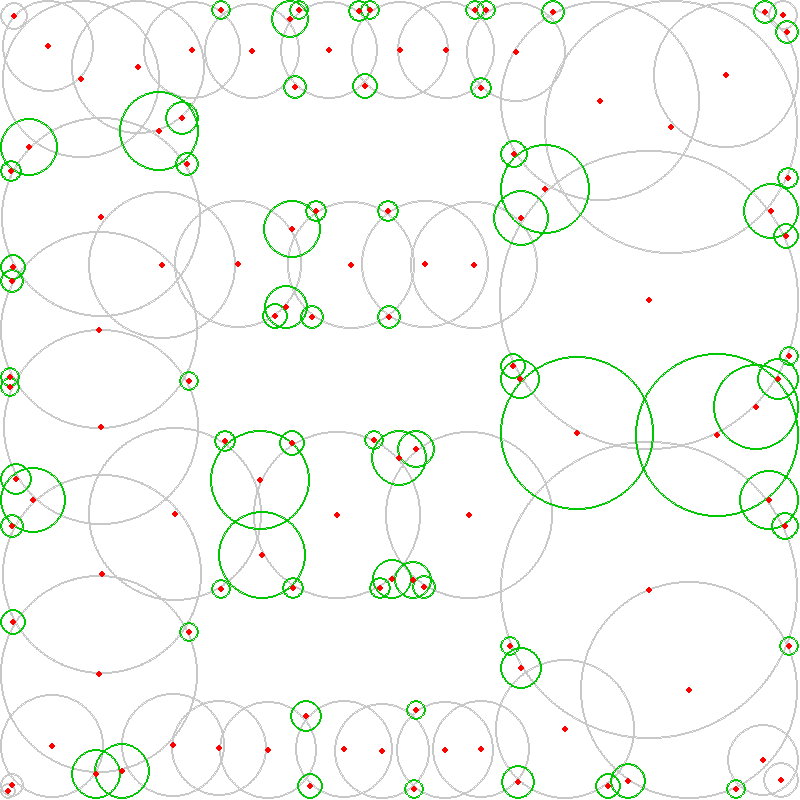
\includegraphics[scale=0.3]{./pics/Samples.PNG}}
	\caption{\label{Samples} Samples got by the algorithm}
\end{figure}

%====================================
% Dual shape and topology roadmap
%====================================

\paragraph{C} \emph{Constructing Topology Roadmap of C-space} \hfill \\
\indent After getting these samples, we can now start to build a structure that captures the topology of the space. 

\indent This phase, like the previous one, has two parts: 1. Construct the dual shape of medial axis samples got from phase one. 2. Simplify the dual shape to a simple graph.

\indent In the first part, constructing the dual shape using only the medial axis sample could break the topology of medial axis. The reason is shown in Figure \ref{badthing}: three balls are all centered on medial axis, but their dual shape will be an empty triangle, which introduces a "hole" in that area. To solve this problem we can try to sample a ball centered at the the radical center after getting an empty triangle, and rebuild the dual shape for these four balls. \cite{radical center} Proving the solution is very simple: if there is no obstacles in that area, the newly sampled ball will cover the space, if there is obstacle, the ball will either not be sampled or not connect three of the balls.

\indent With these balls, we then compute their dual shape, which is formed by some 1-simplices and 2-simplices in 2D. The runtime of computing dual shape will be $O(n^2)$ which is the worst case when doing regular triangulation of weighted points. Although using all balls will avoid problem as in Figure \ref{badthing}, we are making $n$ much larger, which results in a bad runtime of this step.  

\indent One might argue that we can simply get configurations on medial and connect them as a roadmap. However, this roadmap doesn't maintain the topology of \emph{C-space}. At some corners, we will still get triangles which don't have information if there are obstacles inside the triangle. By building the dual shape, this will no longer be a problem.

\indent The second part of this phase can be stated as: retract all connected 2-simplices into one point, reconnect these retracted points with other ones using their previous connection. 

\begin{figure}
	\center{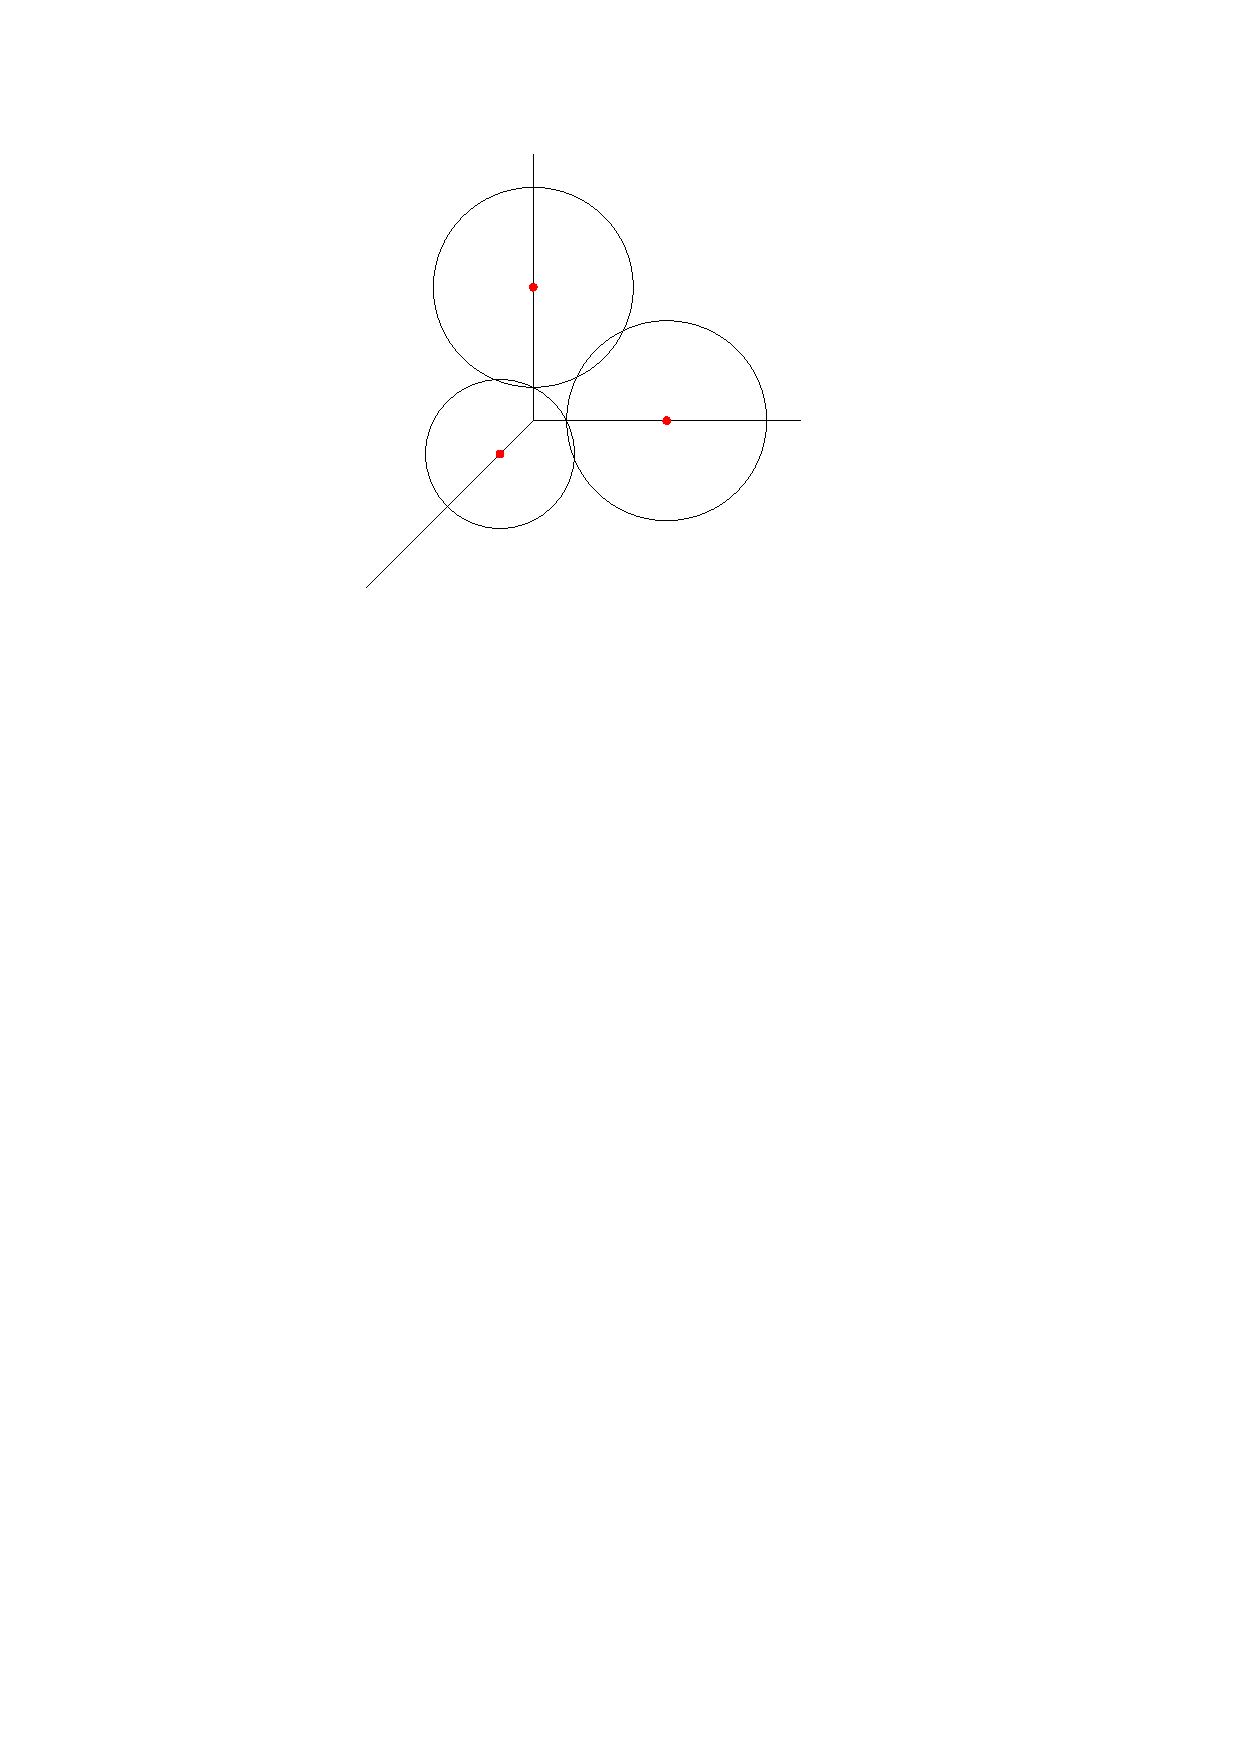
\includegraphics[scale=1]{./pics/badthing.pdf}}
	\caption{\label{badthing}} An example that medial axis samples break the topology structure of the medial axis.
\end{figure}

\begin{figure}
	\center{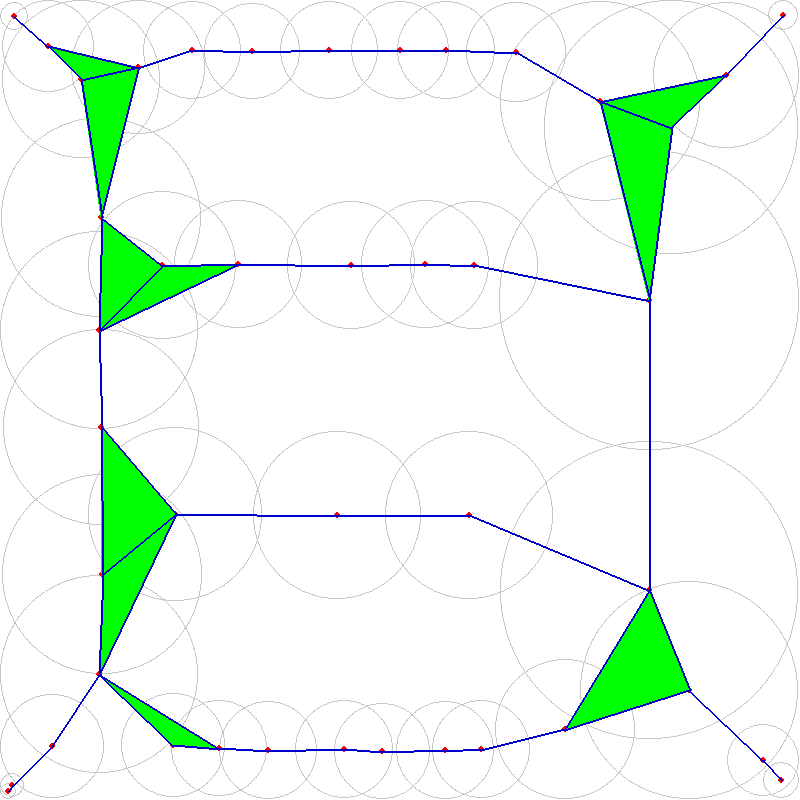
\includegraphics[scale=0.3]{./pics/my_dualshape.PNG}}
	\caption{\label{ourdualshape}} Dual shape of balls generated in phase 1 (centered on medial axis).
\end{figure}

\begin{figure}
	\center{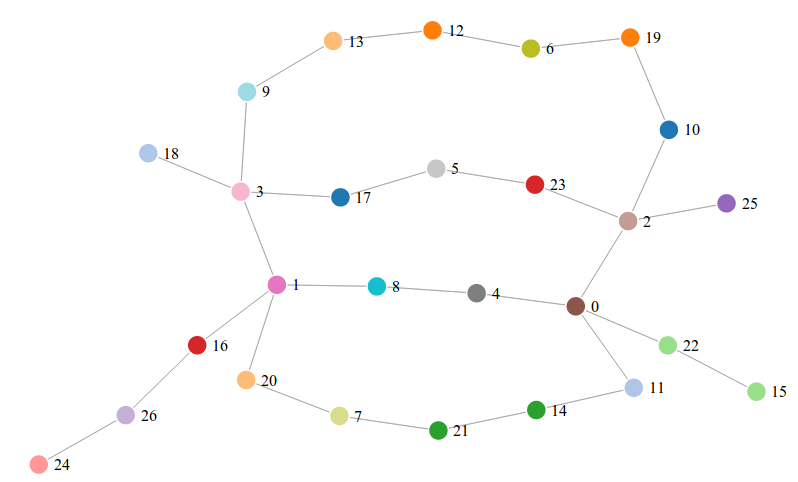
\includegraphics[scale=0.4]{./pics/simplified_graph.png}}
	\caption{\label{simplifiedgraph}} Simplified graph of the dual shape in Figure \ref{ourdualshape}.
\end{figure}

%====================================
% Break graph
%====================================
\paragraph{D} \emph{Breaking A Graph into Loop-free Parts} \hfill\\
\indent After getting the topology roadmap, we technically already have a planner, but still we can simplify it. We now discuss breaking a graph into several components, such that no two components can merge into a new graph without forming a loop. By doing this, a graph is even simplified. Knowing which components are the start and goal configurations in, we can find a path connecting these components immediately. This technique can be a great improve when $C-space$ is very large and traditional \emph{PRM} or \emph{RRT} methods will take a long time to solve.

\indent Let $g_1$ and $g_2$ be two graphs without loops. We say $g_1$ and $g_2$ to be mergeable if: 1. they share at least one common node, 2. the new graph formed by these two graph has no loop. 

\indent Determine if a simple graph has a loop is very easy using the first Betti number $\beta_1$ mentioned in section 2. 

\indent Figure \ref{breakgraph} shows our algorithm to break a graph. The idea behind this algorithm is to take every edges as an initial component, then iterate each component to find and merge with a mergeable component until there is no two mergeable components.

\begin{figure}
\begin{algorithmic}[1] 
  \Function{BreakGraph}{ graph }
  	\State $components \gets EmptySet$
  	\For {$edge \in graph.edges$}
  		\State components.append( new Graph(edge) )
  	\EndFor
  	
  	\State \Return MergeComponents( components )
  \EndFunction
\end{algorithmic}


\begin{algorithmic}[1]   
  \Function{MergeComponents}{components}
  	\State $pq \gets PriorityQueue()$
    \For{$component \in components$}
        \State $pq.push(component, component.size())$
    \EndFor
    \While{ $pq.size() > 1$ }
    	\State $smallest\_component \gets pq.pop()$
    	\State $mergeable\_component \gets$ \emph{find first mergeable component in pq}
		\State $new\_component \gets smallest\_component.merge\_with( mergeable\_component )$
    	\State $components.remove( smallest\_component )$
    	\State $components.remove( mergeable\_component )$
    	\State $pq.remove( mergeable\_component )$
    	\State $components.append( new\_component )$
    	\State $pq.push(new\_component, new\_component.size())$
	\EndWhile
	
    \State \Return $components$
  \EndFunction  
\end{algorithmic}
	\caption{\label{breakgraph}} Breaking a graph into several loop-free components.
\end{figure}

\begin{figure}
	{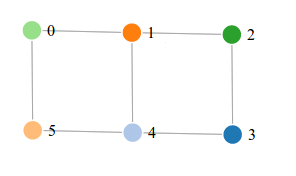
\includegraphics[scale=0.7]{./pics/initial.png}}
	{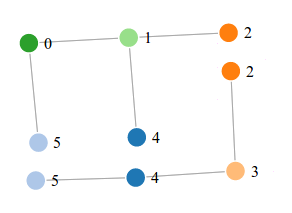
\includegraphics[scale=0.7]{./pics/broken.png}}
	
	{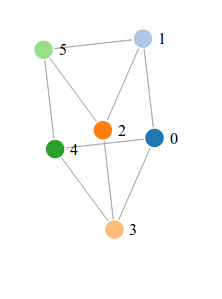
\includegraphics[scale=0.65]{./pics/initial2.png}}
	{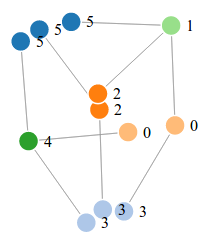
\includegraphics[scale=0.65]{./pics/broken2.png}}\
	\caption{\label{brokengraphs} Some examples of breaking a graph. Graphs are visualized using $d3.js$ $(http://www.d3js.org)$ }
\end{figure}

%====================================
% Path topology
%====================================
\paragraph{E} \emph{Determine Paths Homotopy Class} \hfill \\
\indent A continuous function, or a map, $f: X \rightarrow Y$ is called a \emph{homotopy equivalence} if there is a map $g: X \rightarrow Y$ such that there exist a continuous function $H: X \times [0,1] \rightarrow Y$ with $H(x, 0) = f$ and $H(x,1) = g$.

\indent Besides using those components to plan motions for a large \emph{C-space}, they can also be used to determine if two paths are in the same homotopy class. 

\indent Let $\sigma_1$ and $\sigma_2$ be two paths, with the same start and goal configuration, going through from components $g_1$ to $g_2$ via two nodes $A$ and $B$. $\sigma_1$ and $\sigma_2$ are homotopy equivalent if $A = B$. 

\indent Proof can be found in section 4.

%%%%%%%%%%%%%%%%%%%%%%%%%%%%%%%%%%%%%%%%%%%%%%%%%%%%%%%%%%%%%%%%
%	Properties of Our Algorithm
%
%%%%%%%%%%%%%%%%%%%%%%%%%%%%%%%%%%%%%%%%%%%%%%%%%%%%%%%%%%%%%%%%
\section{Good Properties}\label{properties}
    
  \begin{theorem}
  Let $S_{init}$ be the set of initial random configurations. With minimum radius of $r_{min}$, configurations with clearance larger than $r_{min}$ will be covered, when $|S_{init}| \rightarrow \infty$.
  \end{theorem}
    
  \paragraph{\emph{Proof:}} 
  \indent When the number of initial random configurations approaches infinite, the boundaries of all existing balls are fully covered. So, every configuration not inside any existing balls will be samples as a ball, unless it's less than $r_{min}$ clearance.

  \begin{theorem}
  Let $B$ be the set of ball samples got in phase one. Then $|B|$ is finite.   
  \end{theorem}
  \paragraph{\emph{Proof:}} 
  \indent We restrict balls to have no less than $r_{min}$ radius and new balls to be centered outside existing ones. Assume we partition the space into $r_{min} \cdot r_{min}$ cells in 2D. The number of cells is finite, if the space is finite. Putting balls with exactly $r_{min}$ radius in the centers of these cells will cover the space totally. The number of balls is finite. Phase one will generate balls no more than the number of balls generated in this way. Figure \ref{ourdualshape} shows the dual shape of balls generated by previous phase.
  
  \begin{theorem}
  Let $b \in B$ be an element of $B$, $A$ and $B$ are two configurations in \emph{C-space}. The optimal path $\sigma$ between $A$ and $B$ is in $\bigcup_{b\in B}$ if $\sigma$ has clearance no less than $r_min$. 
  \end{theorem}   
  \paragraph{\emph{Proof}}
  \indent This is a direct conclusion of previous theorem.
  
  \begin{theorem}
  Any path $\sigma$ can be continuously deformed into medial axis. 
  \end{theorem}   
  \paragraph{\emph{Proof}}
  \indent This is the definition of Medial Axis $MA(C_{free})$ being a strong deformation retraction of $C_{free}$.
  
  \begin{theorem}
  Given path $\sigma_1$ and $\sigma_2$, we say they have the same homotopy type if their image in the topology roadmap is the same. 
  \end{theorem}
  \paragraph{\emph{Proof}}
  \indent Let $x$ be a point in the space $X$, $B = \{ b_1, b_2, ..., b_n \}$ be the set of balls centered on medial axis. Define map $H(x)$:
  
  $H(x) = b_i \indent, if \indent |x-b| < |x-b'|, b' \in B$  
 
  \indent This continuous function maps any point in the space to balls centered on medial axis. Dual shape maps any points in the balls to the topology roadmap we build. 
  
  \indent Therefore, if two paths have the same image in the topology roadmap. They have the same homotopy type.
  
  \begin{theorem}
  Let $g_1$ and $g_2$ be two loop-free graphs such that merging their common nodes will produce a new graph with loops, $\sigma_1$ and $\sigma_2$, with the same start and goal nodes, be two paths going from $g_1$ to $g_2$ via common nodes $A$ and $B$. $\sigma_1$ and $\sigma_2$ have different homotopy type if $A \neq B$
  \end{theorem}
  \paragraph{\emph{Proof}}
  \indent Because $A$ and $B$ are two common nodes shared by $g_1$ and $g_2$, if $A \neq B$, merging $g_1$ and $g_2$ will create a graph with a loop going from $A \rightarrow B \rightarrow A$. Since $\sigma_1$ and $\sigma_2$ have the same start and goal nodes, merging them will also create a loop. So $\sigma_1$ and $\sigma_2$ have different homotopy type.

%%%%%%%%%%%%%%%%%%%%%%%%%%%%%%%%%%%%%%%%%%%%%%%%%%%%%%%%%%%%%%%%
%	Experiments
%
%%%%%%%%%%%%%%%%%%%%%%%%%%%%%%%%%%%%%%%%%%%%%%%%%%%%%%%%%%%%%%%%
%\section{Experiments}\label{experiments}
%We now describe the some experiments and their results.

%%%%%%%%%%%%%%%%%%%%%%%%%%%%%%%%%%%%%%%%%%%%%%%%%%%%%%%%%%%%%%%%
%	Conclusions and Future work
%
%%%%%%%%%%%%%%%%%%%%%%%%%%%%%%%%%%%%%%%%%%%%%%%%%%%%%%%%%%%%%%%%
\section{Conclusions and Future Work}\label{conclusions}
We worked hard, and achieved very little.

\bibliographystyle{abbrv}
\begin{thebibliography}{1}

  \bibitem{Book} Steven M. LaValle, "Planning Algorithms", Cambridge University Press, ISBN 0-521-86205-1, 2006.
  \bibitem{UMAPRM} Yeh, Hsin-Yi Cindy, et al. "UMAPRM: Uniformly Sampling the Medial Axis."
  \bibitem{RRT} LaValle, Steven M. "Rapidly-Exploring Random Trees A New Tool for Path Planning." (1998).
  \bibitem{PRM} L. E. Kavraki, P. Svestka, L. E. K. P. Vestka, J. claude Latombe, and M. H. Overmars, “Probabilistic roadmaps for path planning in high-dimensional configuration spaces,” IEEE Trans. Robot. Autom., vol. 12, pp. 566–580, 1996.
  \bibitem{MAPRM} Wilmarth, Steven A., Nancy M. Amato, and Peter F. Stiller. "MAPRM: A probabilistic roadmap planner with sampling on the medial axis of the free space." Robotics and Automation, 1999. Proceedings. 1999 IEEE International Conference on. Vol. 2. IEEE, 1999.
  \bibitem{MAPRM2} S. A. Wilmarth, N. M. Amato, and P. F. Stiller. MAPRM: A probabilistic roadmap planner with sampling on the medial axis of the free space. Technical Report TR98-022, Department of Computer Science, Texas A\&M University, College Station, TX, Nov. 1998.
  \bibitem{DualShape} Edelsbrunner, Herbert. "The union of balls and its dual shape." Proceedings of the ninth annual symposium on Computational geometry. ACM, 1993.
  \bibitem{PointSetShape} Edelsbrunner, Herbert; Kirkpatrick, David G.; Seidel, Raimund (1983), "On the shape of a set of points in the plane", IEEE Transactions on Information Theory 29 (4): 551–559, doi:10.1109/TIT.1983.1056714.
  \bibitem{radical center} "Radical Center", From Wolfram MathWorld -- the web's most extensive mathematics resource. ($http://mathworld.wolfram.com/RadicalCenter.html$)
  \bibitem{PathNonexistance} Z. McCarthy. Bretl, and S. Hutchinson, "Proving path non-existence using sampling and alpha shapes," in IEEE International Conference on Robotics and Automation (ICRA), May 2012.
  \bibitem{betti wiki} "Betti Number", From Wikipedia -- The Free Encyclopedia. ( $http://en.wikipedia.org/wiki/Betti_number$ )    
  \bibitem{Edel Book}Edelsbrunner, Herbert, and John Harer. "Computational topology: an introduction." American Mathematical Soc., 2010. page. 88 - 93.
  \bibitem{alpha betti} Robins, Vanessa. "Computational topology for point data: Betti numbers of α-shapes." Morphology of Condensed Matter. Springer Berlin Heidelberg, 2002. 261-274.
\end{thebibliography}

\end{document}